% ---- FIGURE: mapping-formation frames (single column) ----
\begin{figure}[t]
    \centering
    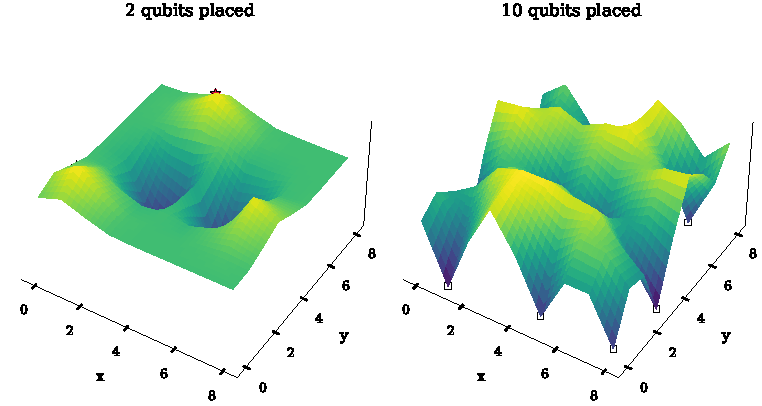
\includegraphics[width=\linewidth]{figures/gaussian_frames.pdf}
    \caption{Formation of a Gaussian-field mapping: the (per-panel normalised)
    score surface $S$ after the indicated number of qubits are committed. White
    squares are committed patches, red stars magic tiles; repulsion carves a well
    at each patch, spacing qubits apart.}
    \label{fig:frames}
    \vspace{-0.5cm}
\end{figure}
